% Created 2021-01-24 Sun 22:50
% Intended LaTeX compiler: pdflatex
\documentclass[11pt]{article}
\usepackage[utf8]{inputenc}
\usepackage[T1]{fontenc}
\usepackage{graphicx}
\usepackage{grffile}
\usepackage{longtable}
\usepackage{wrapfig}
\usepackage{rotating}
\usepackage[normalem]{ulem}
\usepackage{amsmath}
\usepackage{textcomp}
\usepackage{amssymb}
\usepackage{capt-of}
\usepackage{hyperref}
\usepackage{minted}
\hypersetup{colorlinks=true, linkcolor=black, filecolor=red, urlcolor=blue}
\usepackage[turkish]{babel}
\author{Eren Hatırnaz}
\date{16 Aralık 2019}
\title{Yazılım Gündemi - 21\\\medskip
\large 9-15 Aralık 2019}
\hypersetup{
 pdfauthor={Eren Hatırnaz},
 pdftitle={Yazılım Gündemi - 21},
 pdfkeywords={},
 pdfsubject={},
 pdfcreator={Emacs 27.1 (Org mode 9.3)},
 pdflang={Turkish}}
\begin{document}

\maketitle
\tableofcontents \clearpage\shorthandoff{=}

\begin{center}
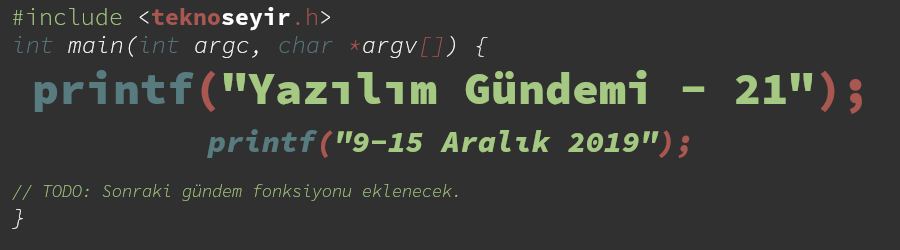
\includegraphics[width=.9\linewidth]{gorseller/yazilim-gundemi-banner.png}
\end{center}

\begin{center}
\href{../20/yazilim-gundemi-20.pdf}{< Önceki Gündem} | \textbf{9-15 Aralık 2019} | \href{../22/yazilim-gundemi-22.pdf}{Sonraki Gündem >}

\href{https://teknoseyir.com/blog/yazilim-gundemi-21-9-15-aralik-2019}{TeknoSeyir'de Oku}
\end{center}

\section{Windows sistemleri etkileyen kritik Git \href{https://github.blog/2019-12-10-multiple-git-vulnerabilities-in-2-24-and-older/}{güvenlik açıkları kapatıldı}}
\label{sec:orgc62081b}
Aslında güvenlik açıkları sadece Windows sistemleri etkilemiyor, aynı zamanda
sisteminizde NTFS olarak formatlanmış bir disk bölümünüz varsa bu açıklarsan
sizde etkilenebilirsiniz. Git geliştiricileri, mümkün olan en kısa sürede Git
sürümlerinizi güncellemenizi öneriyor. Güvenlik açıklarının teknik detayları
başka güvenlik sorunlarına neden olabileceği için henüz yayınlanmamış fakat yol
açtıkları sorunlar hakkında kısa bilgilendirmelere ulaştım. Şöyle ki:

\begin{itemize}
\item \href{https://github.com/git/git/security/advisories/GHSA-2pw3-gwg9-8pqr}{CVE-2019-1348}: \texttt{git fast-import} komutunun \texttt{-{}-export-marks} argümanından
kaynaklanan dosya yollarının üzerine yazmayla ilgili bir güvenlik açığı.
\item \href{https://github.com/git/git/security/advisories/GHSA-4qvh-qvv7-frc7}{CVE-2019-1349}: \texttt{git clone} komutu ile resurcive olarak submodule indirirken
uzaktan kod çalıştırmaya yarayan güvenlik açığı.
\item \href{https://github.com/git/git/security/advisories/GHSA-44fr-r2hj-3f4x}{CVE-2019-1350}: Unutulan bir tırnak işaretiyle \texttt{git clone
    -{}-recurse-submodules} komutunun farklı komutlar çalıştırmasına yol açan bir
güvenlik açığı.
\item \href{https://github.com/git/git/security/advisories/GHSA-39hj-fvvf-mq4f}{CVE-2019-1351}: \texttt{git clone} komutunun, Windows'daki alfabetik olmayan (C,D
yerine 1 ya da Unicode karakter içeriyorsa) mantıksal disk bölümlerinin
üzerine yazmasına neden olan güvenlik güvenlik açığı.
\item \href{https://github.com/git/git/security/advisories/GHSA-5wph-8frv-58vj}{CVE-2019-1352}: \texttt{git clone} işlemi sırasında NTFS Alternate Date Streams ile
ilişkili bir sorun yüzünden \texttt{.git} klasörü içerisindeki dosyaların üzerine
yazmaya neden olan bir güvenlik açığı.
\item \href{https://github.com/git/git/security/advisories/GHSA-589j-mmg9-733v}{CVE-2019-1353}: WSL üzerinde Git kullanırken NTFS'in Shortnames özelliğinden
kaynaklanan bir sorun yüzünden \texttt{git clone} sırasında uzaktan kod çalıştırmaya
imkan sağlayan bir güvenlik açığı.
\item \href{https://github.com/git/git/security/advisories/GHSA-xjx4-8694-q2fq}{CVE-2019-1354}: Windows'daki klasör isimlerinde $\backslash$ işaretinin farklı amaç için
kullanılmasından doğan dosyaların üzerine yazabilmeyi sağlayan bir güvenlik
açığı.
\item \href{https://github.com/git/git/security/advisories/GHSA-4wfr-gwrh-8mj2}{CVE-2019-1387}: Submodule isimlerinin doğrulaması sırasında oluşan hatadan
doğan güvenlik açığı.
\item \href{https://github.com/git/git/security/advisories/GHSA-cj5c-9839-g2ch}{CVE-2019-19604}: \texttt{.gitmodules} dosyasında bir scripti ya da çalıştırılabilir
dosyayı işaret eden komut barındırmaya yarayan bir güvenlik açığı.
\end{itemize}

Görüldüğü gibi güvenlik açıklarının sayısı epey bir fazla, bu yüzden mutlaka
mümkün olan en kısa zamanda Git sürümlerinizi güncelleyin. Eğer yakın bir
zamanda güncelleyemeyecek durumdaysanız şunları yapmaktan kaçının:
\begin{itemize}
\item \texttt{git clone -{}-recurse-submodule} ve \texttt{git submodule update} komutlarını çalıştırmak,
\item Güvenmediğiniz depolar için \texttt{git fast-import} komutunu çalıştırmak,
\item Güvenmediğiniz depoları NTFS formatlı bir disk barındıran sistem üzerinde
clone etmek.
\end{itemize}

Bu güvenlik açıklarını kapatan Git sürümleri ise şu şekilde: v2.24.1, v2.23.1,
v2.22.2, v2.21.1, v2.20.2, v2.19.3, v2.18.2, v2.17.3, v2.16.6, v2.15.4 ve
v2.14.6.
\section{NPM, dosyalara erişim sağlamaya yol açan bir \href{https://blog.npmjs.org/post/189618601100/binary-planting-with-the-npm-cli}{güvenlik açığını kapattı}}
\label{sec:org769f5c3}
Güvenlik açığı hakkında yeterince teknik bilgi sağlanmasa da NPM
geliştiricileri, package.json dosyasının işlenmesi sırasında doğan bir güvenlik
açığı kullanıcının bilgisayarındaki herhangi bir dosyaya erişim ve değiştirme
yetkisi verilmesine neden oluyor. Anladığım kadarıyla bu işlemi yapabilmesi
için paket yayınlayıcısının package.json dosyasına bir takım binary kodlar
eklemesi gerekiyor. Sorun package.json dosyasının işlenmesinden doğduğu için
aynı güvenlik açığı yarn paket yöneticisinde de mevcut. NPM takımı, npm
sistemindeki kayıtlı tüm package.json dosyalarında bu tarz bir açıktan
faydalanan paketleri bulmaya çalışmış fakat bir şey çıkmamış. Tabii ki yine de
gerekli güncellemelerin en kısa zamanda yapılmasını şiddetle tavsiye ediyorlar.
\section{NGINX Rusya ofisi polis tarafından \href{https://www.zdnet.com/google-amp/article/russian-police-raid-nginx-moscow-office/}{basıldı} ve 2 kişi tutuklandı}
\label{sec:org9f95da0}
\begin{center}

\includegraphics[height=3cm]{gorseller/nginx-polis-baskını.png}
\end{center}

NGINX'i hepimiz, şu anda en çok kullanılan web sunucu araçlarından birisi
olarak tanıyoruz, geliştiricisi Igor Sysoev, NGINX'i 2004 yılında açık kaynak
olarak lisanslı şekilde duyurmuştu fakat o zamanlarda henüz NGINX kendisinin
tam zamanlı işi değildi ve Rusya'nın popüler arama motorlarından biri olan
Rambler için çalışıyormuş. Bu haftanın gündemine oturmasının sebebi de bundan
kaynaklı. Geliştirici başka bir firma için çalışırken o firmanın sağladığı
imkanlar ile bu yazılımı geliştirdiği için bir telif hakkı sorunu ortaya çıkmış
ve polis baskını ile kaynak kodlar ve çeşitli belgelere el konulmuş. Aslında bu
durumun yeni ortaya çıkması çok ilginç çünkü geliştirici 2012 yılında verdiği
\href{https://habr.com/ru/company/xakep/blog/136354/}{bir röportajda} (rusça) kendisi de söylemişti "o zamanlar Rambler için
çalışıyordum" diye fakat ilgili firmanın yeni aklına düşmüş herhalde ya da
başka bir takım olaylar var. Ayrıca kodlara el koymaları da ilginç olmuş NGINX
zaten açık kaynak, el koymak için baskın yapmanıza gerek yoktu. Zaten böyle bir
telif hakkı sorunu için polis baskını yapmak ayrı bir saçmalık gibi geliyor
bana. Baskında polisler şöyle mi seslendiler acaba: "Şimdi sakin ol ve elindeki
klavyeyi yavaşça bana doğru uzat evlat!" :)

Tutuklanan kişilerin de NGINX'in yaratıcı Igor Sysoev ve şirketin ortaklarından
biri olduğu yönünde haberler var. Konu \href{https://news.ycombinator.com/item?id=21771144}{HackerNews} ve \href{https://www.reddit.com/r/linux/comments/e9oub4/sorry\_cannot\_find\_good\_related\_subreddits\_to/}{Reddit} gibi platformlarda
yaklaşık bir gün boyunca üst sıralarda kaldı ve geliştiricilerin gündemine
oturdu.
\section{Dart programlama dilinin 2.7 sürümü \href{https://medium.com/dartlang/dart-2-7-a3710ec54e97}{duyuruldu}}
\label{sec:org3fd6f6e}
\begin{center}

\includegraphics[width=.9\linewidth]{gorseller/dart-2-7.png}
\end{center}

Google tarafından geliştirilen, \href{https://github.com/flutter/flutter}{Flutter} isimli hibrit mobil uygulamalar
geliştirmeye yarayan uygulama çatısıyla popülerlik kazanan yine Google
tarafından geliştirilen programlama dili Dart programlama dilinin bu hafta
içerisinde 2.7 numaralı sürümü duyuruldu. Aynı zamanda Dart, bu yıl yayınlanan
GitHub Octoverse raporunda (bkz: \href{../17/yazilim-gundemi-17.pdf}{Yazılım Gündemi - 17}) en hızlı büyüyen birinci
programlama dili seçilmişti. Dille ilgili hiçbir deneyimim yok ama eklenen
özellikleri anlayabildim. O halde 2 özelliğe birlikte bakalım:

\subsection{Eklenti metodları}
\label{sec:org69caa66}
Bu özellik sayesinde artık herhangi bir tip için özel bir fonksiyon
ekleyebileceksiniz. Tip'in sizin tarafınızdan yaratılmış olması da
gerekmiyor. Örnek verecek olursak:
\begin{minted}[breaklines=true,breakanywhere=true,frame=lines, linenos, label=Dart, labelposition=topline]{dart}
extension ParseNumbers on String {
  int parseInt() {
    return int.parse(this);
  }
}

main() {
  int i = '55'.parseInt();
  print(i);
}
\end{minted}
Yukarıda String veri tipine \texttt{parseInt} isminde bir fonksiyon ekledik ve String
içerisine yazılan bir sayının \texttt{int} veri tipine çevrilmesini sağladık.
\subsection{Null Safety}
\label{sec:org89f3727}
Henüz preview aşamasında olsa da faydalı bir özellik. Örnek üzerinden
inceleyelim:
\begin{minted}[breaklines=true,breakanywhere=true,frame=lines, linenos, label=Dart, labelposition=topline]{dart}
class Kisi {
  String ad;
  DateTime dogumTarihi;
  Kisi(this.ad, this.dogumTarihi);

  void tanit() {
    print(ad);
    int dogumYili = dogumTarihi?.year;
    print("${DateTime.now().year - dogumYili} yıl önce doğmuştur");
  }
}
\end{minted}
Örnekte dikkat etmeniz gereken \textbf{?} karakterinin kullanımı. \textbf{?} karakteri ile
yapılan aslında şuydu: \texttt{dogumTarihi} property'sinde değer tanımlıysa year
property'sini getir. Yani doğum tarihinin girilmediği durumlarda \emph{year metodu
bulunamadı} gibi bir takım hatalardan kaçınılmış oldu.


Dart programlama dilinin yeni sürümü ile gelen diğer özellik ve değişiklikler
için konu başlığına eklediğim blog yazını okuyabilirsiniz.
\section{Flutter 1.12 \href{https://medium.com/flutter/announcing-flutter-1-12-what-a-year-22c256ba525d}{duyuruldu}}
\label{sec:orgf1c7129}
Google tarafından Dart programlama dili ile geliştirilen hibrit uygulama
geliştirme çatısının bu hafta 1.12 sürümü duyuruldu. Duyurulan bazı şeyler bu
şekilde:

\begin{itemize}
\item MacOS desteği eklendi. Windows ve Linux desteği de eklenecek.
\item Web desteği beta olarak duyuruldu.
\item Geliştirici ve tasarımcıların birlikte çalışmasını kolaylaştırmak için
Google ve Adobe XD partnerliği duyuruldu.
\item iOS 13'de eklenen Dark mode özelliğine erişebilme desteği,
\item AndroidX desteği,
\item Google Fonts desteği,
\end{itemize}

\url{gorseller/flutter112-macos.gif}

Bu hafta \href{https://teknoseyir.com/durum/1186783}{benim de katıldığım} \href{https://www.meetup.com/tr-TR/GDGTrabzon/events/265973568/}{GDG DevFest '19 Trabzon} etkinliğinde Flutter
1.12'de eklenen MacOS ve Web desteğinin de demosu yapıldı. Açıkcası her ne
kadar Google teknolojileri ilgimi çekmese de mobil uygulamanın aynısın hem
mobilde hem de masaüstü ve web ortamlarında aynı şekilde çalıştığını kanlı
canlı görmek beni şaşırtmadı değil. Sunumu yapan kişinin Flutter 1.12 ile gelen
özellikler hakkında \href{https://medium.com/@sercanyusuf/flutter-interact-all-you-need-to-know-207f5ffccfb9}{yayınlandığı yazıyı da} okumanızı tavsiye ederim.
\section{Android Açık Kaynak Projesine code search \href{https://android-developers.googleblog.com/2019/12/code-search-with-cross-references-for-aosp.html}{web arayüzü eklendi}}
\label{sec:org9d71ba5}
Biliyorsunuz ki Android ilk 1.0 sürümünden beri açık kaynak bir mobil işletim
sistemi. Şu anda Google'ın dağıttığı daha özel bir hali olsa da orijinal
Android kaynak kodları da yine Google tarafından sunulmaktaydı. Fakat bu kaynak
kodlar içerisinde gezinmek o kadar kolay değildi. Şimdi ise yepyeni ve modern
bir arayüze sahip bir proje haline geldi. Üstelik fonksiyonun tanımlandığı ve
kullanıldığı yerleri de göstermek gibi özellikleri de mevcut. İlgili arkadaşlar
mutlaka incelesinler: \url{https://cs.android.com/}
\section{Mikro-kontrolcüler için Qt kütüphanesinin 1.0 \href{https://www.qt.io/blog/qt-for-mcus-1.0}{sürümü yayınlandı}}
\label{sec:org9d07097}
Geçtiğimiz yazılım gündemi yazılarında (bkz: \href{../06/yazilim-gundemi-06.pdf}{Yazılım Gündemi - 6}) bahsettiğim
mikro-kontrolcüler üzerinde Qt kütüphanesi ile kullanışlı ve güzel arayüzler
tasarlamaya yarayan kütüphanenin 1.0 sürümü bu hafta yayınlandı. Maalesef C++
deneyimim pek olmadığı için detaylar hakkında fazla bilgiye sahip değilim.
Bilgi olan arkadaşların yorumlar bölümünde katkılarını bekliyorum. Detaylar ve
rehberler için konu başlığına eklediğim bağlantıya tıklayabilirsiniz.
\section{Visual Studio Code Kasım 2019 (v1.41) \href{https://code.visualstudio.com/updates/v1\_41}{sürümü yayınlandı}}
\label{sec:orgdb7418e}
\begin{center}
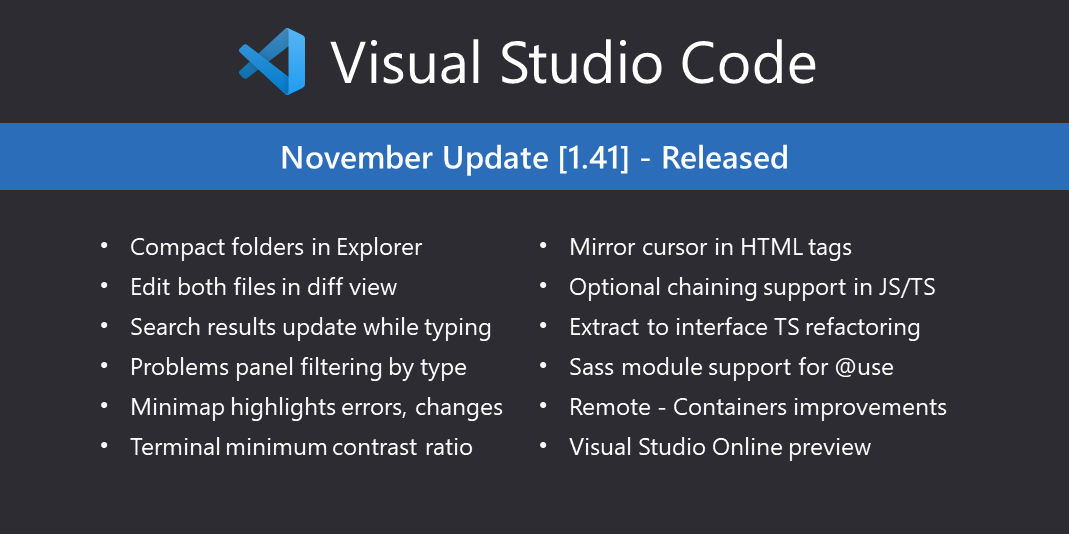
\includegraphics[width=.9\linewidth]{gorseller/vscode-1-41.png}
\end{center}
\section{Yaklaşan Etkinlikler}
\label{sec:org5b01282}
\begin{longtable}{|p{8cm}|l|l|}
\hline
Etkinlik İsmi & Yeri & Tarihi\\
\hline
\endfirsthead
\multicolumn{3}{l}{Önceki sayfadan devam ediyor} \\
\hline

Etkinlik İsmi & Yeri & Tarihi \\

\hline
\endhead
\hline\multicolumn{3}{r}{Devamı sonraki sayfada} \\
\endfoot
\endlastfoot
\hline
\href{https://www.ariteknokent.com.tr/tr/ekosistem/beetech}{Beetech} & İstanbul & 17 Aralık 10:00\\
\href{https://www.eventbrite.com/e/postgresql-de-sharding-fdw-ve-partitioning-tickets-85763158917}{PostgreSQL' de sharding \& FDW ve Partitioning} & Ankara & 17 Aralık 18:00\\
\href{https://www.meetup.com/Teknolot/events/267080760/}{Global AI Bootcamp 2019 Türkiye} & İstanbul & 17 Aralık 19:00\\
\href{https://kommunity.com/software-craftsmanship-turkey/events/panel-yazilimcinin-yolu}{Panel: Yazılımcının Yolu} & İstanbul & 18 Aralık 19:00\\
\href{https://www.eventbrite.com/e/oyun-gelistirme-gunleri-2-tickets-84091625315}{Oyun Geliştirme Günleri 2} & İstanbul & 19 Aralık 12:30\\
\href{https://www.meetup.com/Ankara-Tech-Talks/events/267184427/}{Ankara Tech Talks \& JetBrains - S02E3 - Kotlin Night} & Ankara & 19 Aralık 18:30\\
\href{https://www.meetup.com/Sahibinden-D2D-Events/events/267159689/}{Agile’dan DevSecOps’a giden yol} & İstanbul & 19 Aralık 19:00\\
\href{https://www.meetup.com/Istanbul-Java-User-Group/events/267106749/}{Alternatif JVM'ler ve Java'nın geleceği} & Online & 19 Aralık 19:00\\
\href{https://www.eventbrite.com/e/siber-guvenlikte-kariyer-tickets-85975261321?aff=ebdssbdestsearch}{Siber Güvenlikte Kariyer} & İstanbul & 20 Aralık 18:30\\
\href{https://www.eventbrite.com/e/snort-ile-savunma-keyfi-hacknightsorg-tickets-78022805311}{Snort ile Savunma Keyfi} & Ankara & 20 Aralık 19:00\\
\href{https://www.meetup.com/rladies-ankara/events/267184624/}{Temel R Eğitimi 2} & Ankara & 21 Aralık 12:00\\
\href{https://www.meetup.com/IzmirGophers/events/267057206/}{Go 101 Workshop ve Yazılım Tasarımında Paradigmalar} & İzmir & 21 Aralık 15:00\\
\href{https://www.meetup.com/IBMCloudTR/events/266704608/}{Deploy Java Microservices to OpenShift on IBM Cloud} & İstanbul & 24 Aralık 19:00\\
\href{https://www.meetup.com/ING-\%25C4\%25B0novasyon-Merkezi/events/266639841/}{Bir Yazılım Geliştirici İçin Çeviklik Neden Önemli?} & İstanbul & 27 Aralık 18:30\\
\href{https://www.meetup.com/Facebook-Developer-Circle-Ankara/events/267134880/}{Facebook Developer Circle: Ankara, Advanced React Concepts} & Ankara & 28 Aralık 10:00\\
\href{https://www.meetup.com/rladies-istanbul/events/267184117/}{R ile Zaman Serileri} & İstanbul & 28 Aralık 12:30\\
\href{https://www.meetup.com/Facebook-Developer-Circle-Istanbul/events/267037979/}{PyTorch ile Deep Learning'e Giriş} & İstanbul & 28 Aralık 15:00\\
\hline
\end{longtable}
\section{Diğer Haberler}
\label{sec:orga03a56d}
\begin{itemize}
\item İlk ticari bilgisayar için programlama dili yazan Tony Brooker, 94
yaşında \href{https://www.nytimes.com/2019/12/13/technology/tony-brooker-dead.html}{hayata veda etti}.
\item Google Compute Engine için yeni bir sanal makine ailesi \href{https://cloud.google.com/blog/products/compute/google-compute-engine-gets-new-e2-vm-machine-types}{duyurdu:
E2}.
\item Lincoln Labs: "Uzay araçlarının yazılımları için \href{https://www.reddit.com/r/rust/comments/earm80/lincoln\_labs\_endorses\_rust\_for\_spacecraft/}{Rust kullanılabilir}"
\item Visual Studio 2019 16.4 sürümü \href{https://docs.microsoft.com/en-us/visualstudio/releases/2019/release-notes}{duyuruldu}.
\item Vim 8.2 sürümü \href{https://www.vim.org/vim-8.2-released.php}{yayınlandı}.
\item JDK 14 Erken Erişim sürümü \href{https://jdk.java.net/14/}{yayınlandı}.
\item Crystal programlama dilinin 0.32.0 sürümü \href{https://crystal-lang.org/2019/12/11/crystal-0.32.0-released.html}{yayınlandı}.
\item Python için geliştirilmiş bağımlılık yönetimi aracı Poetry 1.0.0
sürümünü \href{https://python-poetry.org/blog/announcing-poetry-1-0-0.html}{duyurdu}. \href{https://github.com/python-poetry/poetry}{GitHub Deposu}
\item Qt 5.14 sürümü \href{https://www.qt.io/blog/qt-5.14-has-released}{yayınlandı}.
\item Açık kaynak takım için sohbet aracı Zulip, 2.1 sürümünü \href{https://blog.zulip.org/2019/12/13/zulip-2-1-released/}{duyurdu}.
\item Komut satırından JSON görüntülemeye yarayan araç fx, 16.0.0
sürümünü \href{https://github.com/antonmedv/fx/releases/tag/16.0.0}{yayınladı}.
\item Rust ile yazılmış 3D renger kütüphanesi \href{https://leod.github.io/rust/gamedev/rendology/2019/12/13/introduction-to-rendology.html}{duyuruldu}: \href{https://github.com/leod/rendology}{Rendology}.
\item MathSharp, 2.0.0-pre sürümü \href{https://www.nuget.org/packages/MathSharp/}{çıktı}.
\item Barman, 2.10 sürümü \href{https://www.pgbarman.org/barman-2-10-released/}{çıktı}.
\item LibICal 0.1.0 sürümü \href{https://imag-pim.org/blog/2019/12/13/libical-v0.1.0/}{duyuruldu}. \href{https://github.com/matthiasbeyer/libical/}{GitHub Deposu}
\end{itemize}
\section{Lisans}
\label{sec:org5569449}
\begin{center}
\begin{center}

\includegraphics[height=1.5cm]{../../../img/CC_BY-NC-SA_4.0.png}
\end{center}

\href{yazilim-gundemi-21.pdf}{Yazılım Gündemi - 21} yazısı \href{https://erenhatirnaz.github.io}{Eren Hatırnaz} tarafından \href{http://creativecommons.org/licenses/by-nc-sa/4.0/}{Creative Commons
Atıf-GayriTicari-AynıLisanslaPaylaş 4.0 Uluslararası Lisansı} (CC BY-NC-SA 4.0)
ile lisanslanmıştır.
\end{center}
\end{document}
